\documentclass{article}

% if you need to pass options to natbib, use, e.g.:
%     \PassOptionsToPackage{numbers, compress}{natbib}
% before loading neurips_2018

% ready for submission
% \usepackage{neurips_2018}

% to compile a preprint version, e.g., for submission to arXiv, add add the
% [preprint] option:
%     \usepackage[preprint]{neurips_2018}

% to compile a camera-ready version, add the [final] option, e.g.:
     \usepackage[final]{nips_2018}

% to avoid loading the natbib package, add option nonatbib:
%     \usepackage[nonatbib]{neurips_2018}

\usepackage[utf8]{inputenc} % allow utf-8 input
\usepackage[T1]{fontenc}    % use 8-bit T1 fonts
\usepackage{hyperref}       % hyperlinks
\usepackage{url}            % simple URL typesetting
\usepackage{booktabs}       % professional-quality tables
\usepackage{amsfonts}       % blackboard math symbols
\usepackage{nicefrac}       % compact symbols for 1/2, etc.
\usepackage{microtype}      % microtypography
\usepackage{graphicx}
\usepackage{subcaption}
\usepackage{amsmath}

\graphicspath{ {imgs/} }

\title{CS 7180 Milestone 2}

% The \author macro works with any number of authors. There are two commands
% used to separate the names and addresses of multiple authors: \And and \AND.
%
% Using \And between authors leaves it to LaTeX to determine where to break the
% lines. Using \AND forces a line break at that point. So, if LaTeX puts 3 of 4
% authors names on the first line, and the last on the second line, try using
% \AND instead of \And before the third author name.

\author{%
  Nalin Gupta \\
  \texttt{NUID: 001497315} \\
  \And
  Christopher Botica\\
  \texttt{NUID: 001726854} \\
  \And
  Tyler Brown\\
  \texttt{NUID: 001684955} \\
  % Coauthor \\
  % Affiliation \\
  % Address \\
  % \texttt{email} \\
  % \AND
  % Coauthor \\
  % Affiliation \\
  % Address \\
  % \texttt{email} \\
  % \And
  % Coauthor \\
  % Affiliation \\
  % Address \\
  % \texttt{email} \\
  % \And
  % Coauthor \\
  % Affiliation \\
  % Address \\
  % \texttt{email} \\
}

\begin{document}
% \nipsfinalcopy is no longer used

\maketitle

\section{Introduction}

Images taken in low-light conditions are often too dark, noisy, and
distorted to be used in industrial purposes. We propose a deep-learning
model that processes low-light images to improve image brightness and
increase their overall quality. The problem with imaging in low-light
conditions is challenging due to low-photon count and low
Signal-to-Noise (SNR) ratio. These yield very dark and noisy images. The
most common technique to overcome this problem is long exposure shot.
However, this method yields blurry images with the slightest camera shake
or object motion\cite{chen2018learning}. Common post-processing
techniques brighten the image at the expense of image quality. Being able to
``see in the dark'' provides a number of real-world benefits such as
photography, computer vision, and social networking.

\section{Related Work}

In the past, the problem of enhancing low light images has been tackled via
noise reduction. This noise becomes dominant especially in low-light images
due to low SNR. Remez et. al. proposed a deep CNN for noise reduction under
the assumption that this low-light noise belongs to a Poisson
distribution \cite{remez2017deep}.  They used images from ImageNet
\cite{imagenet_cvpr09} as their ground truth data
and added synthetic Poisson noise to simulate corrupted images. Even though
their model outperform the state-of-the art de-noiser ``BM3D'', it does not
scale well to real world images, due to their underlying assumptions.
Furthermore, their model only denoises images but does not brighten them.
Motivated by these downfalls, Chen et. al., proposed an end-to-end CNN,
``See-in-the-Dark'' (SID), which brightens extremely low light images and
removes noise without making any underlying assumptions
\cite{chen2018learning}. However these advances come with the added expense
of collecting large amounts of low
light and bright light images. In the absence of a true vs noisy image
dataset, the team captured scenes using various exposure times to generate
true (bright light) and corrupted (low light) image pairs called
``See-in-the-Dark Dataset'' (SID Dataset
\footnote{https://github.com/cchen156/Learning-to-See-in-the-Dark}). Furthermore,
their model is camera specific and not easily generalizable.\newline

We propose a transferable CNN for image brightening and denoising. Instead
of training our model on actual true (bright light) and corrupted
(low light) image pairs, we use images from the publicly available
RAISE raw images dataset \cite{Dang-Nguyen:2015:RRI:2713168.2713194}. We
use the RAISE raw images dataset as our true images and corrupt these by
simulating low-light conditions for use in our model. We train our CNN on
this synthetic
data to obtain our initial model parameters. A small fraction of the real
images paired from the SID dataset is then used in our transfer learning
\cite{Goodfellow-et-al-2016} approach to update our model parameters.
These model parameters are updated for the particular camera used in the
SID dataset. We then use this model to test on the SID Dataset. In
addition, we aim to test various transfer learning approaches, such as the
traditional transfer learning and zero shot learning \cite{larochelle2008, NIPS2009_3650,socher2013zeroshot}. \newline

The novelty of our approach stems from the idea of ``more for less''. Our
model drastically reduces the overhead costs of data collection by
synthesizing readily available training data (RAISE raw images dataset).
This is
particularly beneficial in domains where collecting images pairs is
expensive/time consuming.

\section{Methods}

Our contributions were to simulate the data and replicate their model
using simulated data.

\subsection{Dataset}

\subsection{Model}

As illustrated in Figure 1, the traditional pipeline takes a corrupted image, and applies the following sequence of modules: Reduce Black Level, Denoising, White Balance, and Gamma Correction. The Black Level refers to refers to the level of brightness at the darkest parts of the image, and is reduced by subtracting the minimum pixel value. Denoising is reduced using common algorithms such as BM3D. White Balance refers to the color balance in the image (i.e., white should be true white) and is corrected by re-balancing the intensities of each color RGB. Finally, Gamma Correction controls the overall brightness of the image. We synthetically generate corrupted images by applying the reverse of this pipeline. Gamma Distortion: decrease the brightness of the image, White Imbalance: skew the color-space by multiplying each level of RGB by a random weight, Poisson Noise: add Poisson noise to the image, Black Level: add a negative bias to the pixel values (i.e., random black level). 

\begin{figure}[ht]
  \centering
  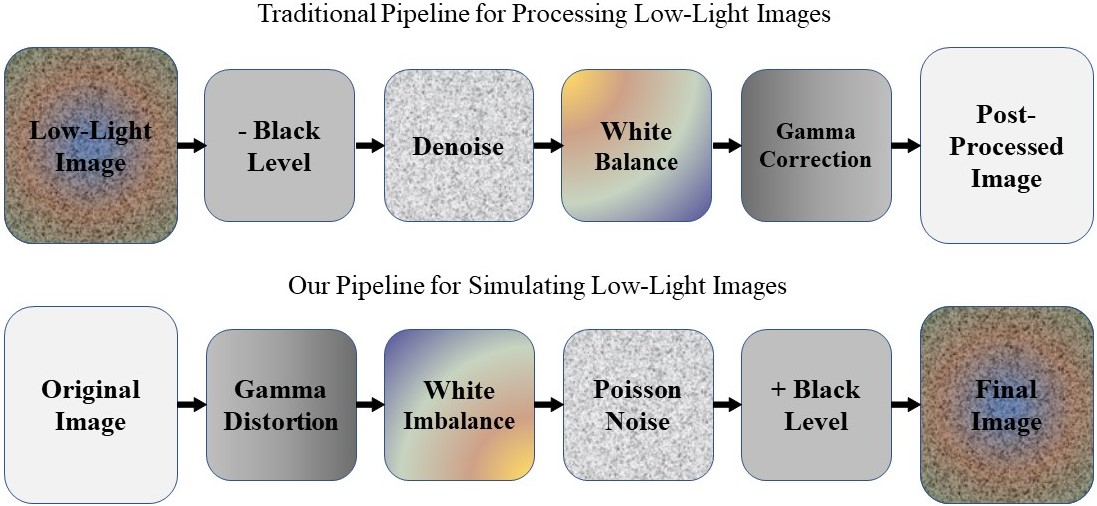
\includegraphics[scale=0.35]{pipeline.jpg}
  \caption{Top: Traditional Pipeline for processing low-light images. Bottom: Our  pipeline to simulate low-light images based on the traditional, only in reverse.}
\end{figure}

Our model is based on the one developed for SID, with the addition of 2 fully-connected layers. Note that we may increase this if training runtime permits. Using the transfer learning approach, we will first train our model on the MIT dataset, then erase the learned weights from the last two fully-connected layers, and retrain on the SID dataset. This is highlighted in our model framework in Figure 2. 

\begin{figure}[ht]
  \centering
  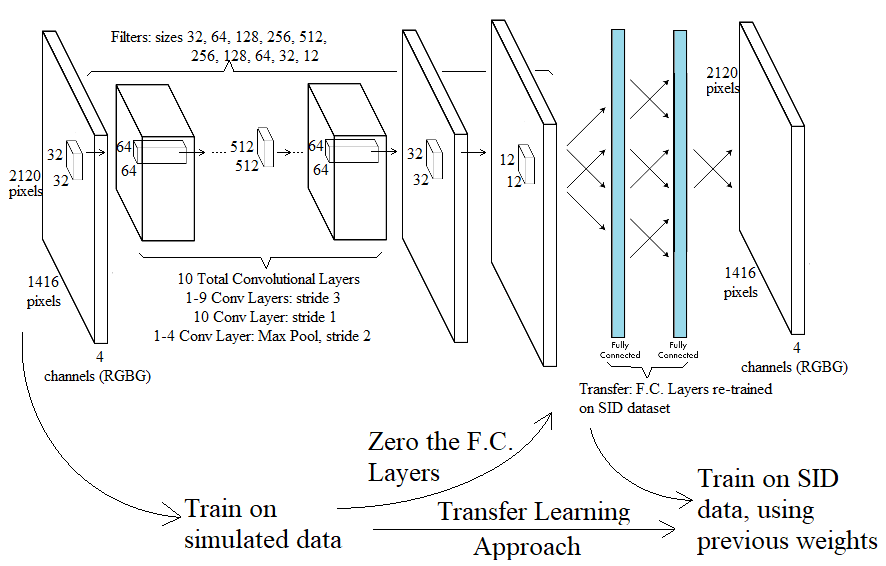
\includegraphics[scale=0.5]{model.png}
  \caption{Our proposed model framework}
\end{figure}

We tried to replicate their model to using other readily
available data such as CIFAR10 \cite{cifar10} and ImageNet
\cite{imagenet_cvpr09}. The CIFAR10 ad ImageNet data is augmented to
simulate properties of the images used by Chen et. al. (2018)
\cite{chen2018learning}. The CIFAR10 and ImageNet datasets are distinctly
different because they are not \textit{raw} images. This means the
dimensionality of CIFAR10 is $32 \times 32 \times 3$ rather than a raw
image which could be $512 \times 512 \times 4$. We not only need to
simulate images but also account for the \textit{change in dimensionality}
across image types.



\subsection{Computational Resources}

Using AWSEducate did not work for us. We were unable to create roles with
IAM authentication so it's really hard or impossible to move data from a
S3 Bucket to an EC2 Instance. We tried to create a $p3.8xlarge$ instance but
these instances are not allowed even though they are listed. Using regular
AWS does work but is costly. Ran a single AWS EC2 $p3.8xlarge$ instance
with 32 CPU, 244 GB of Memory, 4 Tesla V100 GPUs, and 64 GPU Memory. This
costs \$12.24 an hour. This is the amount of GPU Memory requested by the
paper authors as a minimum amount. \newline

We have also been able to use Google Cloud for some of our workload. This
resource is well integrated with Tensorflow. Leading up to Milestone 2,
we extensively used Google Cloud Compute with 2 CPU and 7.5GB of memory
for debugging and working with image datasets; primarily CIFAR10 and
Tiny ImageNet. \newline

In regards to training our model, one of our group members has also
received permission to use computational resources from Lincoln
Laboratory's Super Computer (LLSC) for our project. We are currently
waiting for complete access and expect to be able to use it in the coming
days.

\subsection{Low Light Simulation}

TODO: some theory, maybe Chris?

\begin{figure}[ht]
  \centering
  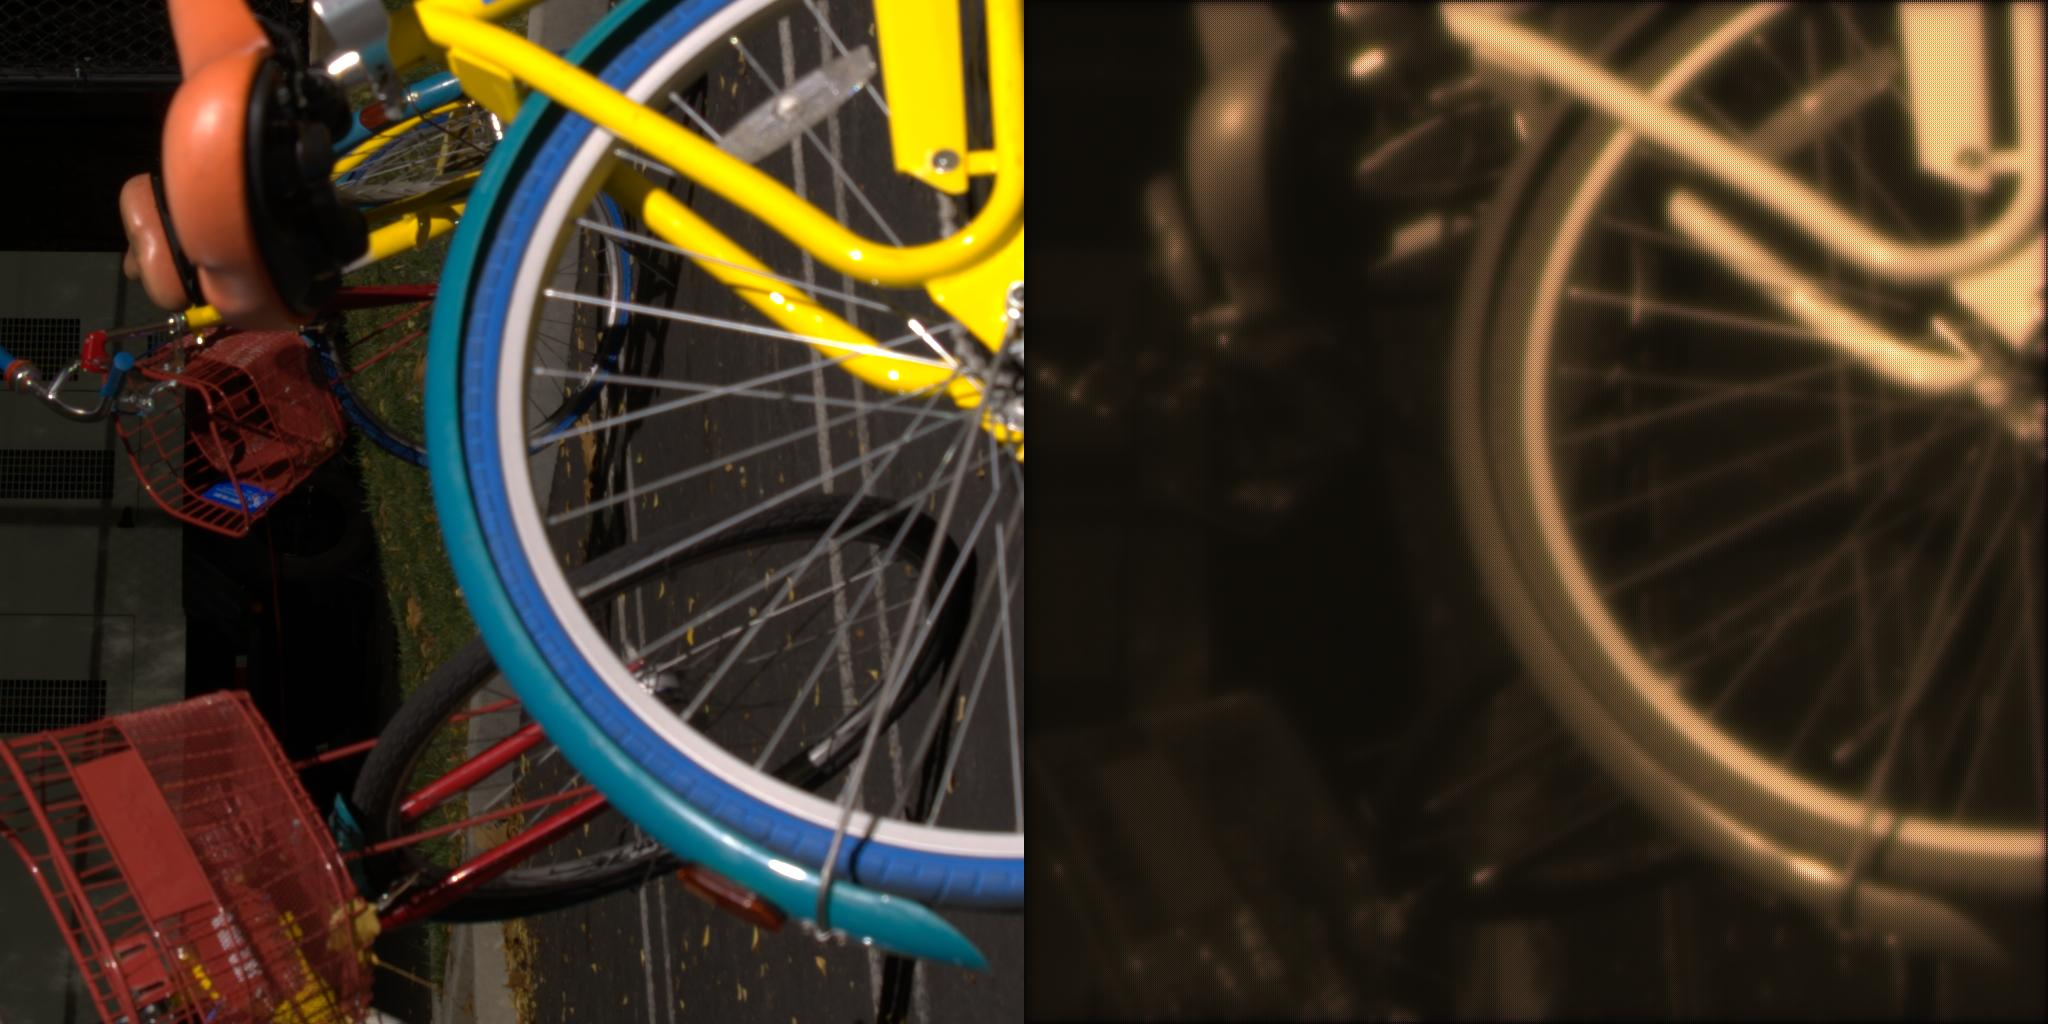
\includegraphics[scale=0.1]{00002_00_train_100}
  \caption{ SID Images in Normal and Low Light Conditions}
  \label{fig:train}
\end{figure}


\section{Experiment}

We experimented on our contributions

\subsection{Model Implementation}

We tried replicating their model and writing a model in parallel to
replicate their functionality. We also tried using the CIFAR10 and
ImageNet datasets as input. The primary issue when replicating their
model related to dimensionality. The RGB images in CIFAR10 and ImageNet
have $m \times n \times 3$ dimensions. Raw images have $m \times n \times 4$
dimensions.

We were able to confirm that output dimensions from Chen et. al.
\cite{chen2018learning} follow the pattern $2m \times 2n \times 3$
irrespective of the image size or type used. During our experiment,
we focused our debugging efforts on understanding whether the dimensionality
of a raw image as an input generated incompatible dimensions with the
target vector after model output. This error resulted in our replicated
model not being able to compute the cost function.

In terms of techniques used, their model is mostly written in a higher
level Tensorflow contribution module called ``slim''. The ``slim''
contribution module does not appear to have any documentation and requires
one to read the module code embedded within Tensorflow. We initially tried
writing a model in parallel using Keras but found that moving from Keras
objects back down to lower level Tensorflow for some blocks within
forward propagation to not be documented well. We then rewrote the
Chen et. al. \cite{chen2018learning} model using only low level Tensorflow
code. This approach has the disadvantage of requiring the dimensions of
all weight matrices to be specified and initialized in a separate function
we called 'initialize\_parameters()'.

These efforts allowed us to understand the dimensionality of both models
at each of the 10 blocks within their forward propagation. We also
experimented with pooling in regards to window size. We also experimented
with strides for convolutional layers with each block. We also added up
to three additional blocks with different parameters in an attempt to
get the output dimensions to match the dimensionality of our input image.

At this point, we have not been able to use RGB images, having
$m \times n \times 3$ dimensions, to work with Chen et. al.
\cite{chen2018learning} model. It is important for us to develop this
capability in order to qualitatively verify that we are correctly augmenting
image data. We are unable to generate images in raw format because
it would require us to know proprietary information about how a camera
generated an image.

In order to generate output for this milestone, we modified images from
Chen et. al. \cite{chen2018learning}, such that

\begin{align*}
  X &= g(y_{train})\\
  Y &= y_{train}
\end{align*}

where function $g$ is an application of artificial noise to a clean
image in $y_{train}$ which is then trained against a corresponding
image where $g$ has not been applied.

\subsection{State of the Art Model Results}

The model used by Chen et. al. \cite{chen2018learning} trains on raw
images for 4,000 epochs. It beats the current state of the art denoising
technique, BM3D. An example of a result for this model is shown in
Figure \ref{fig:train}. A drawback of this model is that it learns a
separate model for each device used to capture the raw images.

\begin{figure}[ht]
  \centering
  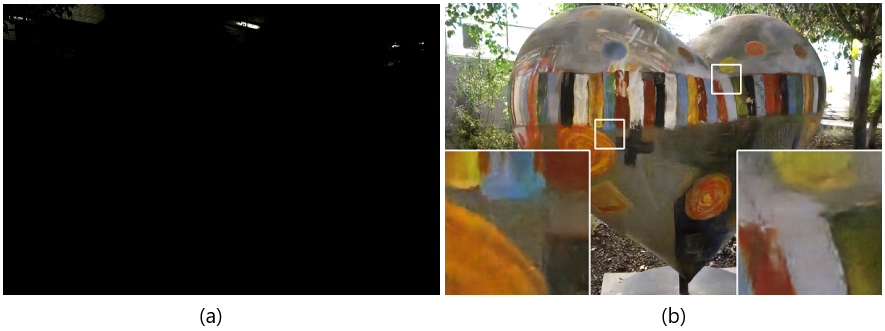
\includegraphics[scale=0.35]{Their_results}
  \caption{ State of the Art Model Results}
  \label{fig:train}
\end{figure}

We can see in Figure \ref{fig:train}, a nearly dark image in sub-figure
(a) is converted to an image shot in normal light conditions; shown
in sub-figure (b).

\subsection{Our Model Results}

\begin{figure}[ht]
  \centering
  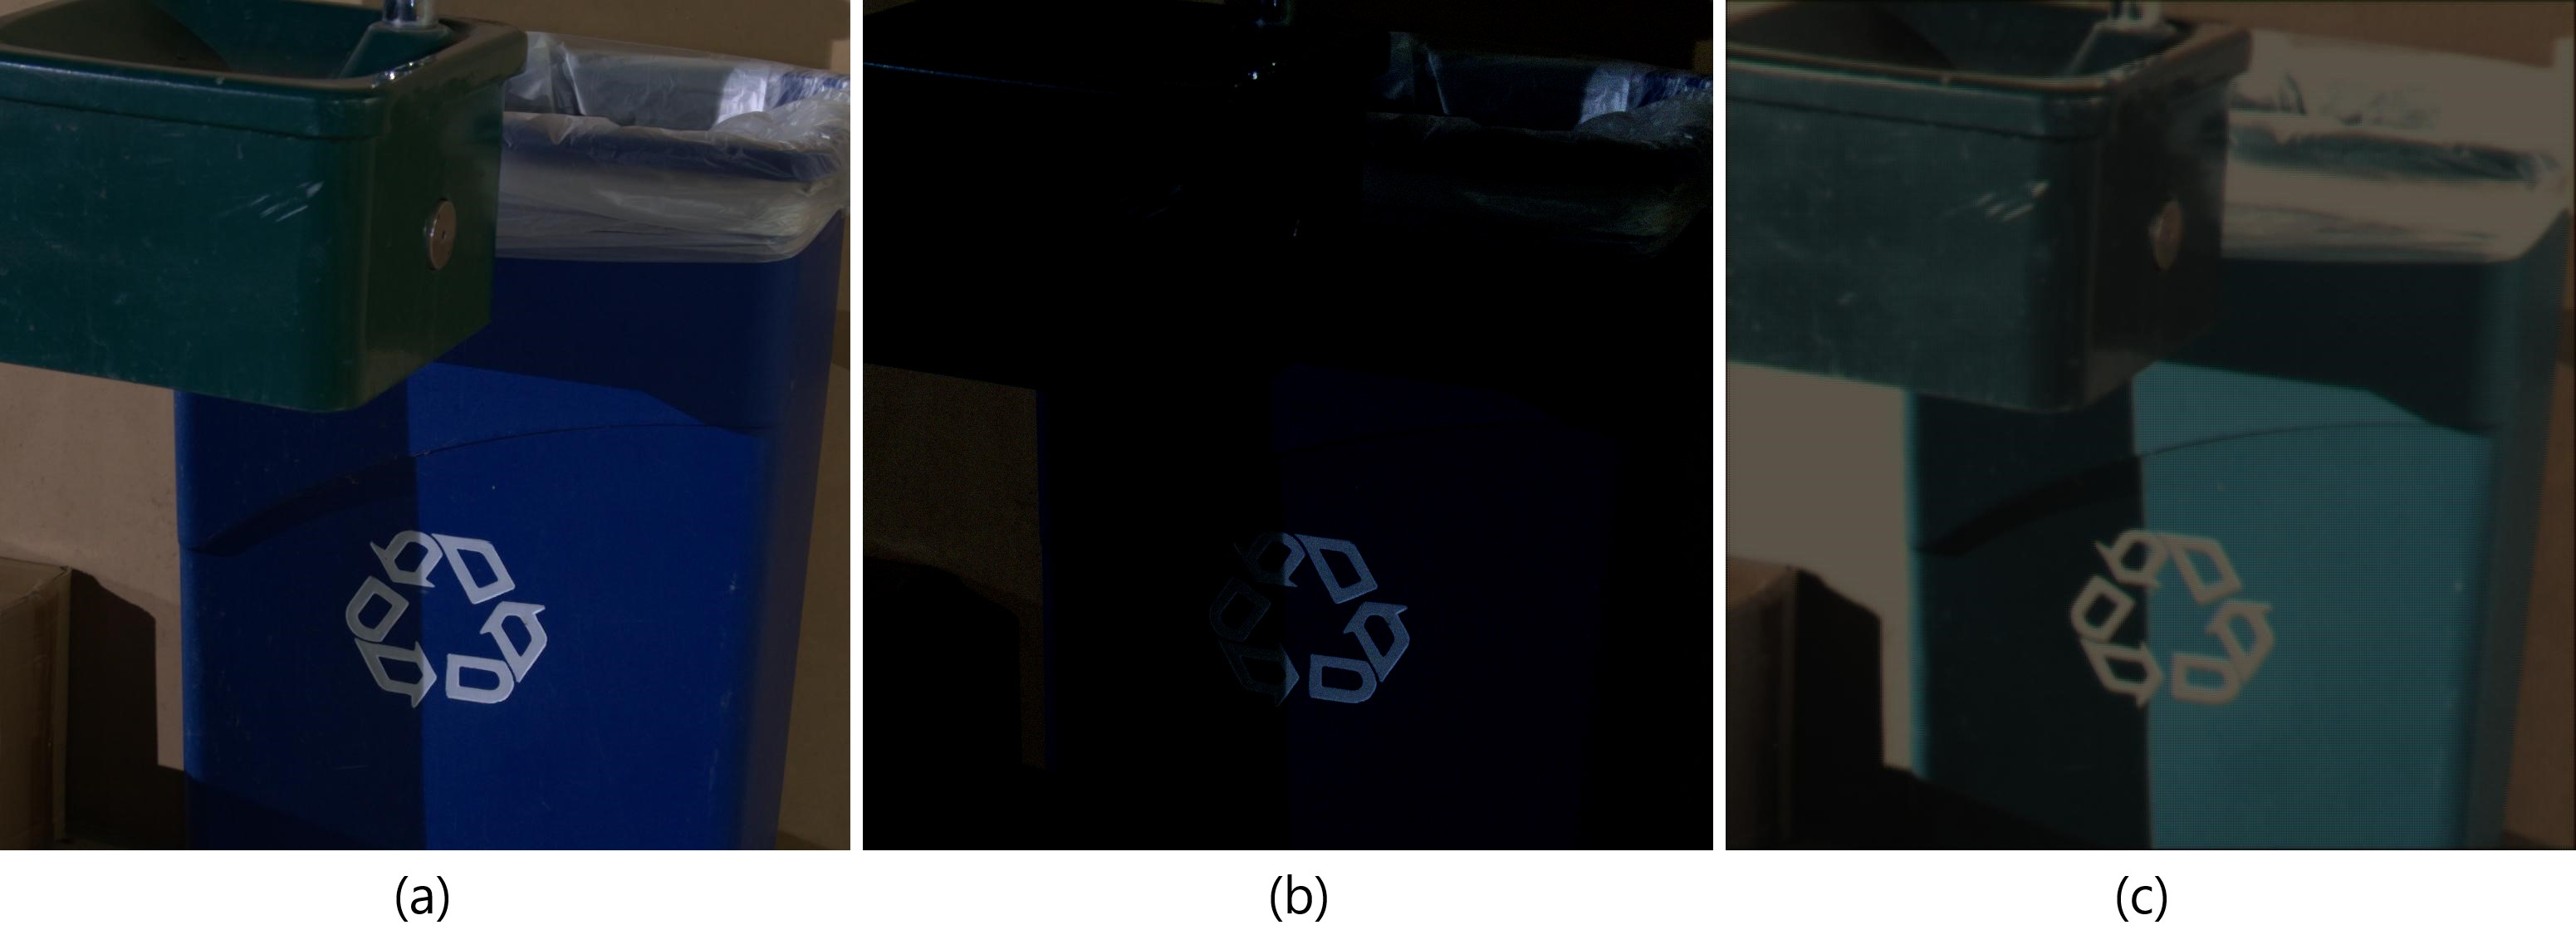
\includegraphics[scale=0.1]{trashcan_original_simmulated_and_our_result}
  \caption{ Predicted Results}
  \label{fig:train}
\end{figure}


\section{Discussion}


\section{Appendix}

\bibliographystyle{unsrt}
\bibliography{references}

\end{document}
